\documentclass[fyp]{socreport}
\usepackage{fullpage}
\usepackage{graphicx}
\usepackage{amsmath, amsfonts}
\usepackage{float}
\usepackage{listings}
\usepackage{color}
\usepackage[table,xcdraw]{xcolor}
\graphicspath{ {./images/} }

\newcommand\norm[1]{\lVert#1\rVert}
\definecolor{dkgreen}{rgb}{0,0.6,0}
\definecolor{gray}{rgb}{0.5,0.5,0.5}
\definecolor{mauve}{rgb}{0.58,0,0.82}

\lstset{frame=tb,
	language=Python,
	aboveskip=2mm,
	belowskip=2mm,
	showstringspaces=false,
	columns=flexible,
	basicstyle={\small\ttfamily},
	numbers=none,
	numberstyle=\tiny\color{gray},
	keywordstyle=\color{blue},
	commentstyle=\color{dkgreen},
	stringstyle=\color{mauve},
	breaklines=true,
	breakatwhitespace=true,
	tabsize=4
}

\begin{document}
\pagenumbering{roman}
\title{Cancelable Biometrics: Analysis and Implementation of a Fingerprint Template Transformation Method}
\author{Arman Kompany Zare}
\projyear{Fall 2023}
\advisor{Dr. Carlisle Adams}
\maketitle
\begin{abstract}
In this report, we analyze, implement, and verify a specific cancelable biometric method from a 2018 research paper \cite{wencheng18cbio}, which is used for transforming fingerprint templates. Our implementation of this method has been solely developed on Python over the course of three months with the help of some open source python libraries. The implementation closely follows the given algorithms on the paper and bears certain advantages in comparison such as improved runtime performance using GPU utilization (powered by NVIDIA CUDA), and all tools involved being fully open source and free to use. The verification of the paper's results was done by running the implementation on the same FVC fingerprint datasets used on the paper, using the same parameter configurations as indicated in their different test cases. In regards to the EER values, different outcomes to those on the paper were achieved as a result, which failed to confirm the claimed fingerprint matching accuracy of this method. However, some of the advantages of our implementation are described in detail and proven within this paper. Our implementation's source code is currently shared on a public repository on Github \cite{project}. 

\begin{keywords}
	Fingerprint, Cancelable Biometrics
\end{keywords}
\begin{implement}
	Python 3, Anaconda, Numba, TensorFlow, Nvidia CUDA, Git
\end{implement}
\end{abstract}

\begin{acknowledgement}
   First and foremost, I would like to thank Professor Carlisle Adams for suggesting this particular research subject, and his continued support and supervision on it. I also appreciate Professor Wencheng Yang, and the other authors of the 2018 paper, for responding to my inquiries regarding their work with helpful explanations and answers. Full credits and acknowledgement goes to the developers and maintainers of the Python libraries used within this project.
\end{acknowledgement}


\tableofcontents 
\listoffigures
\listoftables

\chapter{Introduction}
In today's world, biometrics play a greater role than ever in preserving our digital security and privacy.  Some of the reasons that most people and organizations choose biometrics over static or variable string-based passwords are: Uniqueness, Convenience, and Complexity. However, there is one specific weakness involved with biometric methods, which will be discussed further ahead (under Section 1.2). There exist numerous methods for resolving this weakness which generally fall under the term: Cancelable Biometrics. In this report a specific method \cite{wencheng18cbio} which is used for fingerprint biometric data, will be discussed and analyzed, along with a documentation on its implementation, yielded results and performance comparison.
\section{Advantages of Biometric Data}
The Uniqueness advantage comes from the fact that when it comes to biometrics, especially fingerprints, almost no two individuals possess the same biometric information. So there are no overlaps in case of comparisons. On the other hand, there is a slim chance that two people in the world would coincidentally share the same static password for their applications or accounts, which would lead to security issues if one of their passwords gets compromised.

Regarding Convenience, it is obvious that biometric information do not necessarily need to be remembered by a person, and are perfectly portable since they are literal parts of that person's own body. On the other hand, complex passwords may be difficult to remember and misinputs could occur while entering them in. Even sometimes, said complex passwords or hashes are so large in data size that they need to be carried around by flash or external drives.

Naturally, the data complexity of a single fingerprint or piece of biometric data surpasses the complexity of an average static password by a great margin. As it will be discussed further later in this report, approximately 2.5 Megabytes worth of data is required for representing a single encoded fingerprint template. Meanwhile an average static password (32 characters) is represented by a mere 32 Bytes of data. At first glance, there may be a space cost disadvantage, but in return the exponentially increased complexity will make it near impossible to reconstruct biometric data through exhaustive search.

\section{The Problem: Irrevocability}
In spite of the advantages mentioned above, static passwords hold at least one important advantage over biometric data, and that is their revocability. In case of a credential leak, the exposed user can easily revoke their password and have it replaced by a new one, and as a result, the leaked password will hold no leverage in future compromises on the same user.

On the other hand, if biometric data, such as a fingerprint get compromised, it will be forever exposed and there will be no way to have it revoked and replaced like a static password. Additionally, the risk for the biometric data to be used in future attacks will remain indefinitely.

\section{The Solution: Cancelable Biometrics}
Fortunately for us, there are a plethora of methods which cover the irrevocability weakness. These solutions fall under the category of Cancelable Biometrics. In general, the method converts a fingerprint into a certain data structure referred to as a template, which represents the fingerprint's minutiae data with great accuracy. Then the method transforms the template using a public key into a transformed template. Afterwards, the transformed template and its respective public key are saved to a database. In case the database gets hacked into, the attacker wouldn't be able to retrieve the original template through the public key and the transformed template. In addition, the transformed template and its respective public key are revocable. Meaning that the exposed data could be easily removed from the database, and be replaced by a new public key from which another completely different transformed template could be generated.

\subsection{Solution Outline}
\label{sol}
The process behind Cancelable Biometrics methods usually involves two generic stages: Enrolment and Verification. The following is a rough explanation of the whole process and its stages.

\subsubsection{Enrolment}
In the Enrolment stage, the Target fingerprint which is supposed to be used as reference for future comparisons gets scanned, and we get a grayscale picture of the fingerprint scan as a result. Next, we need to detect all the valid minutiae points on the fingerprint image, and create an Initial Fingerprint Template (IFT) using said minutiae. The IFT is composed of extracted minutiae data under a number of different schemes. From this point on, is where the most crucial process begins to occur. Using a set of algorithms designed for this specific Cancelable Biometric method, we will transform the IFT into an Transformed Fingerprint Template (TFT) using a psudeo-randomly generated Public Key. Finally, the TFT along with its respective Public Key which was used to generate it, will be stored in memory.

\subsubsection{Verification}
Afterwards, in the Verification stage, our Query fingerprint will be scanned and converted into another IFT using the same schemes and standards based on its minutiae data. Then using the same public key, the IFT will be transformed into a TFT. The Query fingerprint's TFT will then be compared with the Target fingerprint's TFT using a series of comparison methods. Ultimately, using a final score derived from the comparison methods and a predetermined score threshold, we will determine whether the two fingerprints match or not.

\begin{figure}[H]
	\centering
	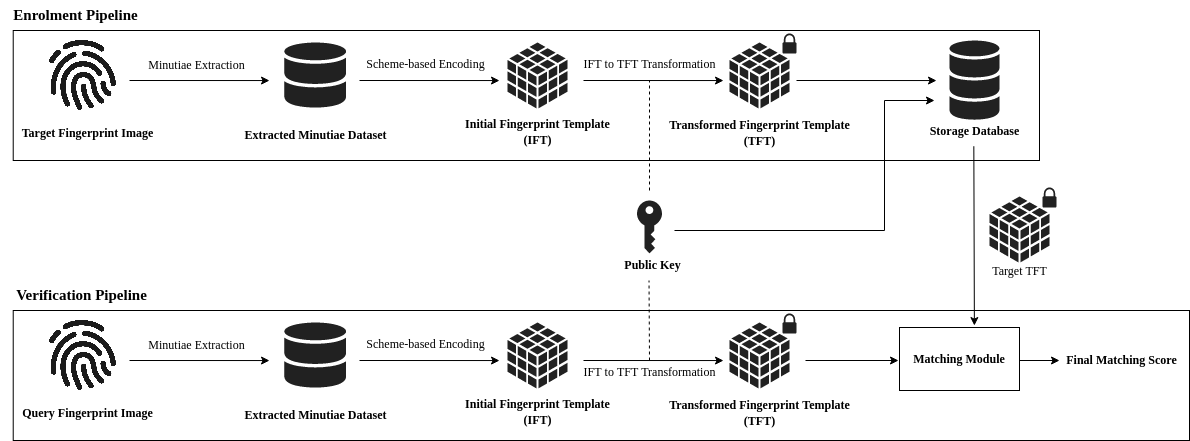
\includegraphics[width=1\textwidth]
	{General_Pipeline}
	\caption{A simplified diagram of the Enrolment and Verification pipelines}
\end{figure}

\subsection{Solution Properties}
Ofcourse, in order for both security and accuracy to be guaranteed, two main requisites must be met in the design a Cancelable Biometric method. One is the irreversibility of the process, in which the IFT gets transformed into the TFT. The other is the comparability of the Target fingerprint's TFT with the Query fingerprint's TFT, hence the differences in the Target and Query IFT must be somewhat preserved in their respective TFTs.

\subsubsection{Irreversibility}
In the case of an intrusion, the worst case scenario would be the compromise of the TFT and Public Key pair. In this case, the infiltrator should not be able to obtain the IFT from the TFT and Public Key by any means other than brute force. For a function to guarantee this attribute, it must preferably be a non-injective function (not one to one), and non-invertible. The input element of this function must be also large enough for exhaustive search to be near impossible. For instance a hash function such as SHA-512, is a good example of an irrevertible function. 

\subsubsection{Comparability}
An irrevertible function such as a hash function may seem to be a good candidate for our purpose at first glance. But when it comes to biometric input, the smallest differences in input data could result in very different and incomparable outputs after being put through something such as a hash function.

Therefore we need a function or transformation that could preserve the small initial differences and render the results comparable. In Chapter 2, a few of these functions, which are relevant to the main algorithm of our study, will be discussed.

\chapter{Preliminaries}
Before we get to the full analysis of the Yang method \cite{wencheng18cbio}, a few basic definitions and concepts will be briefly covered. After a brief explanation of the Yang method, some of its exclusive advantages over other methods in Cancelable Biometrics will be listed. Moreover at the end, the irreversibility and comparability criterias of the IFT to TFT transformations will be demonstrated.


\section{Concepts and Definitions}
\subsection{Minutiae Points}
The exterior of a human fingertip is a pattern of interleaved ridges and valleys. At its local level, important features called minutiae, can be found in fingerprint patterns. In this context, minutiae refers to the various ways that said ridges can be discontinuous. \cite{maltoni22fing}

\begin{figure}[H]
	\centering
	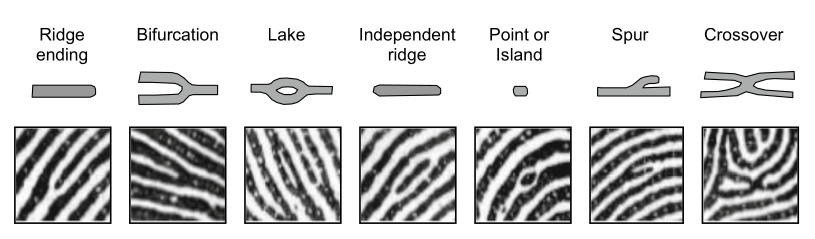
\includegraphics[width=0.65\textwidth]
	{minutiae_types}
	\caption{Seven most common minutiae types}
\end{figure}

\newpage The points in which these discontinuities or changes in ridge pattern occur, are referred to as minutiae points. Minutiae points possess several inherent attributes, but we will only need a few of them for our purposes. Each minutiae point has the following primary attributes include: X-Y cartesian coordinates, minutiae orientation, minutiae type, and a confidence score.

\begin{figure}[H]
	\centering
	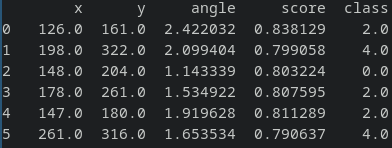
\includegraphics[width=0.4\textwidth]
	{minutiae_pandas}
	\caption{A list of detected minutiae points and their attributes}
\end{figure}

The cartesian coordinates are the pixel coordinates of the minutiae point's location on the fingerprint input image. The orientation of a minutiae, is the direction it is heading towards, or in other words the direction of the line tangent to the ridge at that point. The minutiae type is an integer enumeration of the seven most common types of minutiae as referred to in Figure 2.1. The confidence score, is the probability of that minutiae point being a legitimate minutiae point, according to the FingerFlow framework, which we will discuss in the next chapter.

\subsection{Delaunay Triangulation}
Considering a set of discrete points $P$ on a euclidean plane, a three-point subset:

\begin{center}
	$\{p_1, p_2, p_3\} \subset P$
\end{center}
 is considered a Delaunay Triangle, if and only if no other point in $P$ is inside the circumcircle of the three-point subset. \cite{delaunay34trig}
 
\begin{figure}[H]
	\centering
	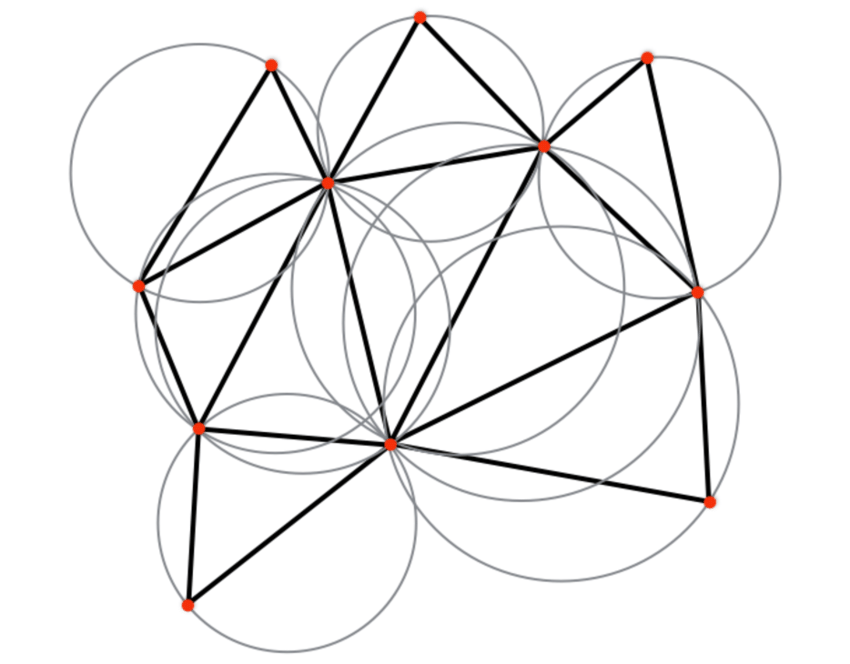
\includegraphics[width=0.35\textwidth]
	{delaunay}
	\caption{A set of points subjected to Delaunay Triangulation}
\end{figure}

After deriving all feasible Delaunay Triangles from the points in $P$, we end up with a connected graph of neighboring triangles with no intersecting edges. There are many algorithms with which to perform Delaunay Triangulation with:

\subsubsection{Voronoi Algorithm}
Given a set of $n$ discrete points $P = \{p_1, p_2, ..., p_n\}$ on a Euclidean plane, the plane is segmented into $n$ non-overlapping partitions dedicated to each point in $P$. Each of these partitions is referred to as a Voronoi cell.  Every Voronoi cell $C_k$, consists of every point on the plane for which its respective point $p_k$ is the closest site. Meaning the distance of any arbitrary point within $C_k$ is minimal from itself to $p_k$ than to any other point $p_i \ne p_k$. The set of all Voronoi cells, make up a Voronoi diagram.

\begin{figure}[H]
	\centering
	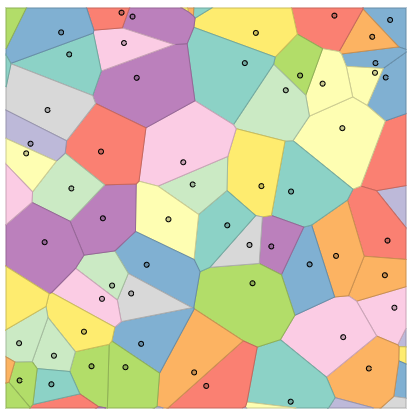
\includegraphics[width=0.4\textwidth]
	{voronoi}
	\caption{A Voronoi diagram consisting of Voronoi cells and their respective points}
\end{figure}

The borders of these Voronoi cells, refered to as Voronoi edges, are constructed by creating the perpendicular bisector of the line between two points respectively and blending them. Finally, the Delaunay Triangulation of $P$ is then created by connecting the points of all neighboring Voronoi cells. The Yang method originally uses the Voronoi algorithm to derive the Delaunay Triangles from the set of minutiae points on a fingerprint. But there is another easier to implement algorithm which was used in our implementation instead.

\subsubsection{The Bowyer-Watson Algorithm}
In computational geometry, the Bowyer-Watson algorithm is an incremental algorithm for deriving all possible Delaunay Triangles from a set of points in N-dimensional Euclidean space. The pseudo-code is fully described in \ref{code:a1}. The complexity for this algorithm is $O(n log(n))$ if implemented efficiently, and $O(n^2)$ in a normal sub-optimal implementation. The Python implementation of the Bowyer-Watson algorithm was readily available from a Python package named \texttt{delaunay-triangulation} \cite{delgit}, which was imported and used in our code.

\begin{figure}[H]
	\centering
	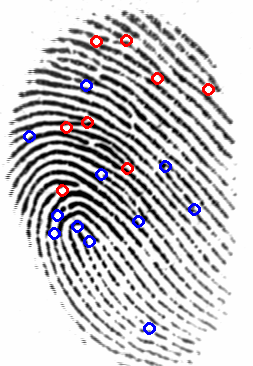
\includegraphics[width=0.2\textwidth]
	{minutiae_points}
	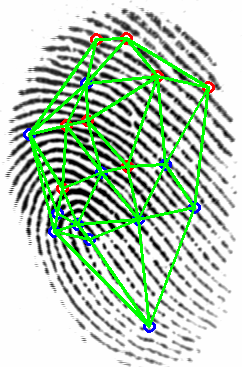
\includegraphics[width=0.191\textwidth]
	{minutiae_del}
	\caption{Minutiae points on a fingerprint and its Delaunay Triangulation}
\end{figure}

\section{The Yang Method}
\subsection{Brief Outline}
The Yang method's outline follows from general outline described in \ref{sol}, and includes the mentioned Enrolment and Verification phases. The generation of the IFT from the fingerprint image, is done separately in parallel under two different schemes: The Polar Coordinate-based scheme and the Delaunay Triangulation-based scheme.

The Polar IFT, which is an array of vectors with zero and one entries, is then transformed using the Feature Decorrelation Algorithm (FDA) (which will be discussed in Chapter 3), and then projected into a lower dimension using a projection matrix pseudo-randomly generated from a seed. The seed used to generate the pseudo-random projection matrix, is a part of the Public Key associated with the TFT. Every vector in the Polar IFT, is essentially based around a reference minutiae point and its polar coordinate-based relations with other minutiae points within a certain predefined radius. Therefore within the Polar IFT, there's a vector dedicated to every minutiae point, since every vector is created by setting a minutiae point as the origin point.

The Delaunay IFT, is essentially an array of all Delaunay Triangles encoded and quantized into binary numbers, based on attributes such as side length, the angle between two sides of the triangle, the minutiae type of the triangle vertices, and orientation differences between two vertices. Thereafter, the Delaunay IFT is permutated into the Delaunay TFT by converting each encoded triangle in the IFT from binary to integer, and adding it to another integer which is generated based on a predetermined integer $\phi$. The $\phi$ number is another part of the Public Key associated with the TFT.

After the two IFTs of the target fingerprint are obtained, we obtain the two IFTs of the query fingerprint using the same Public Key (same projection matrix and $\phi$). Then the similarity scores of the respective IFTs are calculated (\texttt{SC\_MAX} for the Polar IFTs, and \texttt{SD} for the Delaunay IFTs), normalized, and put into a Final Score formula for giving the finalized similarity score of the two fingerprints.

\begin{figure}[H]
	\centering
	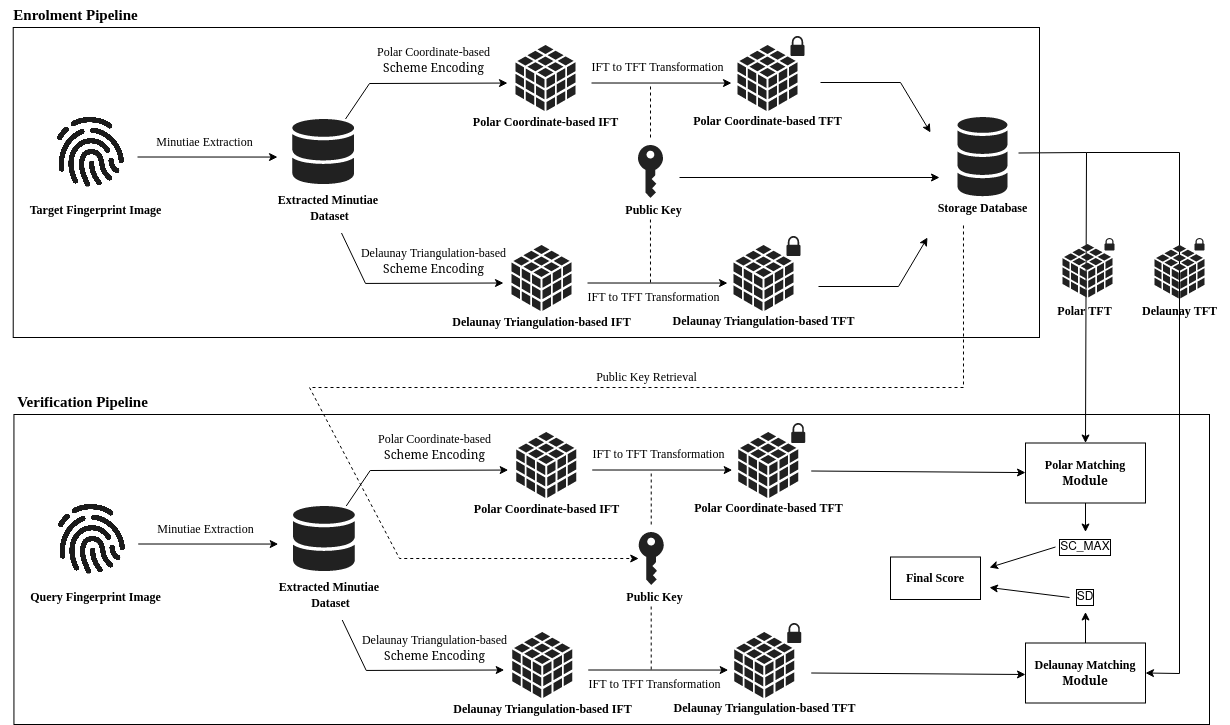
\includegraphics[width=1.1\textwidth]
	{Specific_Pipeline}
	\caption{Full Enrolment and Verification pipeline diagram of the Yang method}
\end{figure}

\subsection{Advantages}
The main contributions of the Yang method compared to the previous works in cancelable biometrics, include the following advantages:

\subsubsection{Reduced Non-Linear Distortion}
Since the Yang method's IFT and final result depend on a combination of the Polar Coordinate-based and Delaunay Triangulation-based schemes, the impact of non-linear distortion, which would lead to recognition inaccuracy being reduced. Roughly speaking, non-linear distortion results from systems in which the output signal is not exactly proportional to the input signal. 

For instance a cause of non-linear distortion would be to have a system which solely relies on the Polar Coordinate-based scheme for the generation of its IFT, which would result in the system not taking into account the minutiae that are located far away from the reference minutiae. That is because, in the Polar Coordinate-based scheme, only minutiae that are placed within a certain limited radius of the reference minutiae are taken into account and used to generate the IFT. Therefore, compared with the system that solely uses a Polar Coordinate-based scheme, higher recognition accuracy is achieved.

\subsubsection{ARM Attack Invulnerability}
The ARM attack, otherwise known as Attack via Record Multiplicity, is an exploit which results from the compromise of several TFTs and their respective generative parameters (the Public Key in our case), and leads to the full or partial generation of the original IFT. A main reason that a lot of Cancelable Biometrics methods suffer from the ARM attack is due to feature correlation. To propagate this issue, a FDA is implemented within the method, so that in the process of the IFT to TFT transformation, the feature vectors within the IFT become uncorrelated in regards to another. Without any correlation between said features in the IFT, the attacker wouldn't have enough data to determine the original IFT.

\subsection{Guarantee of Irreversibility}
\subsubsection{Polar Coordinate-based Scheme}
The irreversibility of the IFT to TFT transformation is guaranteed through the random projection $F$ performed on the IFT vectors. 

\begin{center}
	$F: \mathbb{C}^{n} \to \mathbb{C}^m$ where $n \ge m$: $F(x) = Ax$
\end{center}

In our case, the projection matrix $A$ is composed of pseudo-randomly generated entries based on a seed. According to basic linear algebra fundamentals, since the projection matrix $A$ is not a square matrix, it is therefore not invertible. Therefore it is not possible to derive $F^{-1}$ except through exhaustive search. Hence irreversibility is guaranteed due to the involvement of random projection within the IFT to TFT transformation within the Polar Coordinate-based scheme.

\subsection{Guarantee of Comparability}
\subsubsection{Polar Coordinate-based Scheme}
The irreversibility of the IFT to TFT transformation is guaranteed, but what about its comparability? Will the characteristics of the IFT vectors in regards to each other be preserved after performing random projection on them? Fortunately, the answer is yes, thanks to the Johnson-Lindenstrauss (JL) Lemma \cite{lind84lem}:

\begin{center}
	Lemma: For any $0 \le \epsilon \leq 1$ and any integer $p$, let $n$ be a positive integer such that: $n \ge \frac{4 ln(p)}{\epsilon^2 / 2 - \epsilon^3 / 3}$.
	
	Then for any set $\mathbb{S}$ of $p = |\mathbb{S}|$ data points in $\mathbb{R}^N$, there is a map $f: \mathbb{R}^N \to \mathbb{R}^n (N \ge n)$, such that for all $x, y \in \mathbb{S}$:
\begin{equation}
	(1- \epsilon) \norm{x-y}^2 \leq \norm{f(x) - f(y)}^2 \leq (1+ \epsilon)\norm{x-y}^2
\end{equation}

\end{center}

Overall, the JL lemma states that our IFT vectors in $\mathbb{R}^N$ vector space can be embedded into a lower dimension vector space $\mathbb{R}^n$, such that the difference between any two pair of vectors in the IFT will also be approximately maintained in between their respective pair in the TFT after the random projection is performed on the vectors.



\chapter{Algorithm and Implementation}
This chapter will include the full description of the Yang method and the generations of its IFTs and TFTs. In addition, we will go over the list of tools and frameworks utilized for our implmentation and the reason behind the selection of said tools. We will also go over the instructions for running the code, and the advantages of our implementation.

\section{The Algorithm in Full Detail}
First we begin by obtaining all minutiae and their attributes from the fingerprint image.  As a result we will obtain a set of $N$ minutiae $M = \{m_0, m_1, ..., m_{N-1}\}$ within that image. Every minutiae $m_i \in M$ can be represented by its respective vector $m_i = (x_i, y_i, \theta_i, t_i)$, where $x_i$ and $y_i$ respectively represent the $x$ and $y$ coordinates of the minutiae $m_i$ on the fingerprint picture, $\theta_i$ represents the minutiae orientation, and finally $t_i$ represents the minutiae type. $\theta_i$ ranges between $(0, 2\pi)$, and $t_i$'s value is represented by single bit, signifying whether it is a ridge ending minutiae type or not. We choose to base $t_i$ around the ridge ending minutiae type, because it's the most commonly seen type of minutiae by a great margin compared to other minutiae types. 

\subsection{Generation of the IFTs}
With the minutiae data on hand, we begin generating the IFTs both under the Polar Coordinate-based scheme and the Delaunay Triangulation-based scheme.

\subsubsection{Polar Coordinate-based IFT}
Under this scheme, the final IFT ($C = \{P(m_i)\}_{i=0}^{N-1}$) is an array of vectors with 0 and 1 entries. Each IFT vector $P(m_i)$ is created based on a minutiae point $m_i$ which is used as an origin point. Now let's assume we want to derive $P(m_0)$, we would first have to take minutiae point $m_0$ as reference and calculate the three attributes $(\rho_i, \alpha_i, \beta_i)$ of the other minutiae with respect to $m_0$ as the origin point. 

First off, only minutiae points that fall within a radius $R$ (= 300 pixels) of point $m_0$ are taken into account. Moreover, every other minutiae point's data relative to $m_0$ consists of three attributes. The radial distance $\rho_i$, which implies the distance from selected minutiae $m_i$ to the reference minutiae $m_0$, which ranges from: $0 \le \rho_i \le R = 300$.

Next, we have the radial angle $\alpha_i$, which is the polar angle of minutiae point $m_i$ with respect to $m_0$ as the origin point. The third and last attribute, is the absolute minutiae orientation difference $\beta_i$, between between $m_0$ and $m_i$. Both $\alpha_i$ and $\beta_i$ range from: $0 \le \alpha_i, \beta_i \le 2\pi$.

After the $(\rho_i, \alpha_i, \beta_i)$ triplet for every minutia $m_i \neq m_0$ is obtained, it's time to perform quantization on the three attributes. We assume that the step sizes for $\rho_i$, $\alpha_i$, and $\beta_i$ are $s_{\rho}$, $s_{\alpha}$, and $s_{\beta}$, where $5 \leq s_{\rho} \leq 20$ and $\pi/12 \leq s_{\alpha}, s_{\beta} \leq 2\pi/9$. Then we quantize the polar space around $m_0$ into a 3D cube containing $l_C = L \times S \times H$ cells, where $L = \lfloor R / s_{\rho} \rfloor$, $S = \lfloor 2\pi / s_{\alpha} \rfloor$, and $H = \lfloor 2\pi / s_{\beta} \rfloor$. The cell in which minutia point $m_i$ is located in the 3D cube is $(\rho^q_i, \alpha^q_i, \beta^q_i)$, where $\rho^q_i = \lfloor \rho_i / s_{\rho}\rfloor$, $\alpha^q_i = \lfloor \alpha_i / s_{\alpha} \rfloor$, and $\beta^q_i = \lfloor \beta_i / s_{\beta} \rfloor$. By doing so, we eventually get the vector $P(m_0)$ of length $l_C$, which consists of '1' and '0' entries, which is obtained by concatenating all the rows of cube cell values together in one line. The '1' indicates that one or more quantized minutiae points belong in that corresponding cube cell.

The size of any vector $P(m_i) \in C$ depends on the value of $l_C$, which itself depends on the step sizes for the triplet attributes. The smaller the step sizes, the bigger $l_C$ will get and the more accurate our method becomes. And with our defined boundaries for step sizes, the largest $l_C$ can get, is 34560. To finish this section up, we repeat the same steps mentioned above for all other $m_i$, until we get all other $P(m_i)$ and obtain the full Polar Coordinate-based IFT ($C = \{P(m_i)\}_{i=0}^{N-1}$).



\subsubsection{Delaunay Triangulation-based IFT}
First we start by performing Delaunay Triangulation on all minutiae points in $M$, through either the Voronoi or the Bowyer-Watson algorithm. After all triangles are extracted, we need to go over every triangle $\triangle m_1m_2m_3$ and extract certain attributes from it for further processing. The IFT ($D$) under this scheme, is also similar to the Polar Coordinate-based IFT, in the fact that it is also an array of vectors with zero and one entries, with each vector dedicated to a triangle.

Suppose we're processing the $\triangle m_1m_2m_3$ triangle. There are four attributes $(\alpha_i, l_i, h_i, t_i)$ we need to take into account. First one is $\alpha_i$, which is the size of the largest angle of the triangle, its value is ranged between $0 \le \alpha_i \le 2\pi$. Second and third one are $l_i$ and $h_i$, which are respectively the lengths of the larger and smaller edges of the $\alpha_i$ angle. Both are ranged between $0 \le l_i, h_i \le 300$. Finally, there's $t_i$ which is supposed to represent the minutiae types of the three vertices of the triangle using three bits. First bit is dedicated to the minutiae type of the largest angle's vertice, second and third are dedicated to the minutiae type of the vertices positioned on the larger and smaller edges of the triangle.

At this point, all attributes other than $t_i$ (since it is already a three bit binary vector) need to be quantized. Similar to what we did in the Polar Coordinate-based IFT, the quantization step sizes are set to be $s_{\alpha}$, $s_l$, and $s_h$, which are respectively ranged at $\pi/12 \leq s_{\alpha} \leq \pi/9$, and $15 \leq s_l, s_h \leq 25$. To each attribute, the minimum amount of bits to cover all possible quantization values will be dedicated. For instance, if the value of $\alpha^q_i$ ranges between 0 and 9, then 4 bits will be dedicated to $\alpha^q_i$. The quantized value of each attribute is calculated as follows: $\alpha^q_i = \lfloor \alpha_i / s_{\alpha}\rfloor$, $l^q_i = \lfloor l_i / s_l\rfloor$, and $s^q_i = \lfloor h_i / s_h\rfloor$. Finally we convert each quantized attribute into binary, and concatanate every binarized attribute into a single list which we will refer to as $f^q_{m_1m_2m_3}$. The same should be done with every other triangle to achieve the entirety of our IFT set ($D$).

\begin{center}
	Example:
	
	$[\alpha^q_i, l^q_i, h^q_i, t_i]$ = [10,7,3,[0,0,1]] $\to$ [[1,0,1,0], [0,1,1,1], [0,0,1,1], [0,0,1]] = $f^q_{m_1m_2m_3}$
\end{center}

\subsection{Transformation of the IFTs into TFTs}
With both Polar ($C$) and Delaunay ($D$) IFTs being generated, we move on to transforming them into their respective TFTs.

\subsubsection{Polar Coordinate-based TFT}
The transformation of the Polar IFT ($C$), involves subjecting each of its vectors to Feature Decorrelation and Random Projection. By the end of the process, we will have an array of complex valued vectors which will be stored for further use.

First we need to put each $P(m_i) \in C$, through the Feature Decorrelation Algorithm, or optionally, its extension which is referred to as the Enhanced Feature Decorrelation Algorithm. Overall, the enhanced version allows for tighter security at the expense of performance and matching accuracy. A larger value of $L_S$ in the enhanced algorithm makes it more difficult to revert from $S_j^\prime$ to $S_j$, but at the same time would lower matching accuracy.

\begin{figure}[H]
	\centering
	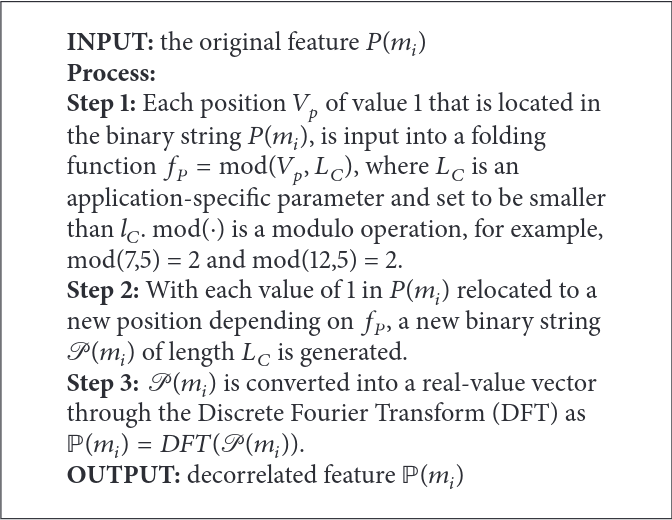
\includegraphics[width=0.48\textwidth]
	{FDA}
	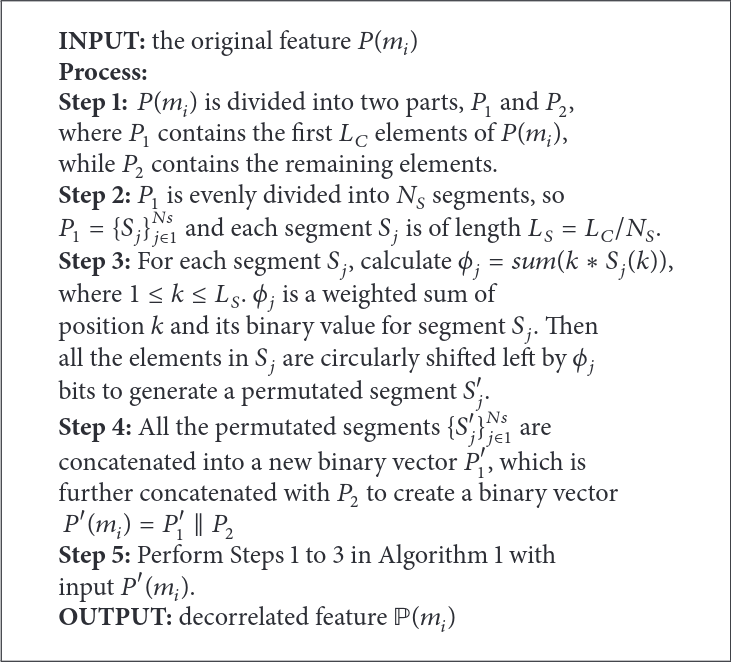
\includegraphics[width=0.48\textwidth]
	{EFDA}
	\caption{The Feature Decorrelation Algorithm (Left) and its Enhanced version (Right)}
\end{figure}

After acquiring the decorrelated complex valued vector $\mathbb{P}(m_i)$ from either of the Feature Decorrelation Algorithms, we will have to project it to a lower dimension $Y$ using a random projection matrix $\mathbb{M}$:

\begin{center}
	$\widehat{P}(m_i) = \mathbb{M} \times \mathbb{P}(m_i)$
\end{center}

 The random projection matrix itself is deterministically generated by a predetermined seed, which is a part of the public key used for the IFT to TFT transformation. The lower $Y$ is, the stronger the irreversibility gets. But in return, we will end up with poorer matching accuracy. After we repeat the same procedure with all $P(m_i) \in C$, we obtain our Polar Coordinate-based TFT: $\widehat{C} = \{\widehat{P}(m_i)\}^{N-1}_{i=0}$.

\subsubsection{Delaunay Triangulation-based TFT}
Given the Delaunay TFT $D$ and each of its vectors $f^q_{m_im_jm_k}$, we aim to permute each of them, and place them each in a lengthy binary vector by their resulting integer representation. First, we convert each quantized attribute in $f^q_{m_im_jm_k}$, which are $\alpha^q_i$, $l^q_i$, $h^q_i$, and $t_i$ into integers using the $int(\cdot)$ function, and obtain the largest integer out of them: $\mathbb{B} = max(f^q_{m_im_jm_k} = [int(\alpha^q_i), int(l^q_i), int(h^q_i), int(t_i)])$. Next, we generate the feature code $f^c_{m_im_jm_k}$ using the following formula, and another part of our public key $\phi$ which is a predetermined positive integer:

\begin{equation}
	\mathbb{Y} = \mathbb{B} + \phi
\end{equation}
\begin{equation}
	f^c_{m_im_jm_k} = \mathbb{Y}^3 int(\alpha^q_i) + \mathbb{Y}^2 int(l^q_i) + \mathbb{Y}^1 int(h^q_i) + \mathbb{Y}^0 int(t_i)
\end{equation}

After obtaining the integer feature code $f^c_{m_im_jm_k}$, we concatenate the entirety of $f^q_{m_im_jm_k}$ into one binary string, convert it to integer, and add it to $f^c_{m_im_jm_k}$, which we will refer to as the Index Number of $f^q_{m_im_jm_k}$. After obtaining all the Index Numbers of each existing $f^q_{m_im_jm_k} \in D$, we then create a zero vector $\widehat{D} = {0,0,...,0}$ that has great length. In our implementation we used a length of $2^{20}$. Next, based on each Index Number we've retrieved from each $f^q_{m_im_jm_k} \in D$, we replace a '0' by '1' in $\widehat{D}$. 

For example if an Index Number is 12763, we will replace the 12763th element in $\widehat{D}$ by '1'. In case of a collision, we shall let the '1' remain. In case the Index Number is larger than than the length of $\widehat{D}$, we will use $mod(Index Number, length(\widehat{D}))$ to determine a feasible Index Number. Thus, $\widehat{D}$ on its own will become our Delaunay TFT.

\subsection{Obtaining the Polar and Delaunay Matching Scores}
Given two TFT sets, one belonging to the Target Fingerprint $(\widehat{C}_T, \widehat{D}_T)$ conceived during the Enrolment stage, and the other belonging to a Query Fingerprint $(\widehat{C}_Q, \widehat{D}_Q)$, we can compare them together and derive definitive scores which will be used for Fingerprint matching down the line.

The matching score resulting from the comparison of the Polar IFTs $\widehat{C}_T$ and $\widehat{C}_Q$, is referred to as \texttt{SC\_MAX}. The other matching score derived from the comparison of the Delaunay IFTs $\widehat{D}_T$ and $\widehat{D}_Q$, is referred to as \texttt{SD}. Both \texttt{SC\_MAX} and \texttt{SD} are ranged between 0 and 1. We will need both to calculate the \texttt{Final\_Score} which is also ranged between 0 and 1.

\subsubsection{Calculating \texttt{SC\_MAX}}
In order to derive \texttt{SC\_MAX}, we plug in every possible pair of vectors $\widehat{P}_T(m_i) \in \widehat{C}_T$ and $\widehat{P}_Q(m_j) \in \widehat{C}_Q$, into the following formula, in order to derive a list of \texttt{SC} values:

\begin{equation}
	\mathtt{SC} = 1 - \frac{\norm{\widehat{P}_T(m_i) - \widehat{P}_Q(m_j)}_2}{\norm{\widehat{P}_T(m_i)}_2 + \norm{\widehat{P}_Q(m_j)}_2}
\end{equation}

Finally, we obtain \texttt{SC\_MAX}, by finding the maximum value in the list of all derived \texttt{SC}s

\subsubsection{Calculating \texttt{SD}}
To obtain \texttt{SD}, we calculate the correlation coefficient of the $\widehat{D}_T$ and $\widehat{D}_Q$ by using the following formula:

\begin{equation}
	\mathtt{SD} = \frac{\sum_{k=1}^{L} (\widehat{D}_{Q,k} - \overline{\widehat{D}_Q}) (\widehat{D}_{T,k} - \overline{\widehat{D}_T})}{\sqrt{\sum_{k=1}^{L} (\widehat{D}_{Q,k} - \widehat{D}_Q)^2 \sum_{k=1}^{L} (\widehat{D}_{T,k} - \widehat{D}_T)^2}}
\end{equation}

In which $L$ is the length of both $\widehat{D}$ arrays (=$2^{20}$ in our implementation), and $\overline{\widehat{D}}$ represents the mean value of said array. Also, the equivalent of the formula above can also be found in the MATLAB programming language as a function referred to as the \texttt{corr2()} function \cite{corr2}. 

\subsubsection{Calculating \texttt{Final\_Score}}
After calculating \texttt{SC\_MAX} and \texttt{SD}, we can finally attribute a matching score to a pair of Target and Query fingerprints. The basic formula for \texttt{Final\_Score} is as follows:

\begin{equation}
	\mathtt{Final\_Score} = (\rho_C \times \mathtt{SC\_MAX}) + ((1- \rho_C) \times \mathtt{SD})
\end{equation}

The variable $\rho_C$ signifies a score multiplier between 0 and 1, which varies depending on whether we'd want to rely more on the Polar or Delaunay scheme for matching the fingerprints. More emphasis is put on the Delaunay scheme the closer it is to 0, and vice versa more emphasis it put on the Polar scheme the closer it is to 1. 

However, we would use a more elaborate formula when there are more than one comparisons involved, which is usually the case when we're working with a database of fingerprints, in which we can have many choices for picking a pair of fingerprints:

\begin{equation}
	\mathtt{Final\_Score} = (\rho_C \times norm(\mathtt{SC\_MAX})) + ((1- \rho_C) \times norm(\mathtt{SD}))
\end{equation}

Where $norm(\cdot)$ resembles a Min-Max normalization function. Before we use the more elaborate formula, we need to normalize the list of all derived \texttt{SC\_MAX} and \texttt{SD} with the normalization function and then plug in the respective normalized \texttt{SC\_MAX} and \texttt{SD} in the formula. We will discuss the uses of \texttt{Final\_Score} for deriving fingerprint matching data in Chapter 4.

\section{Tools and Implementation}
One of the main challenges of implementing the Yang method was having to implement the whole method from scratch. Because unfortunately, the authors of the article under analysis did not put any links or references to their own implementation on their article. Upon further investigation, it was discovered that they've used paid frameworks such as VeriFinger for minutiae extraction and MATLAB for processing the extracted data. Due to budget limitations, it was not possible for us to use said proprietary software. Therefore we would have to resort to free open source solutions.

\subsection{Python}
For this project and our implementation needs, Python (version 3.9+) was our number one choice. Mainly because Python, due to its simple syntax and numerous open source easy to use libraries, is meant for quick prototyping and implementation of any concept or method. Had any other language been chosen, it would have taken far more than four months to implement the whole method and derive results from it.

\subsubsection{Anaconda}
Anaconda itself, is a Python distribution which is mainly meant for scientific programming purposes such as Data Science or Machine Learning. One specific feature of Anaconda which was vital to introducing GPU utilization to our implementation, is the ability to create isolated Python environments. In an environment it's possible to have Anaconda use a specific version of Python and Python packages so that compatibility between them for their intended purposes is guaranteed.

\subsubsection{FingerFlow}
FingerFlow is a python framework for extracting fingerprint minutiae and their respective properties directly from images as input, and returns the minutiae data as a Pandas dataframe \cite{fingerflow}. FingerFlow itself is based around two other Machine Learning and Deep Learning frameworks named TensorFlow and Keras respectively. It is also capable of utilizing CUDA drivers via TensorFlow's capabilities to speed up the minutiae detection.

For it to work, we need to supply it with a few prebuilt .H5 formatted model files named CoarseNet, FineNet, ClassifyNet, and CoreNet, which are provided as links in the FingerFlow project's GitHub repository page. FingerFlow is also capable of matching fingerprints and providing us with a matching score. In Chapter 4, we will analyze FingerFlow's performance when it's utilizing the CPU versus when it utilizes the GPU.

\subsubsection{NumPy}
The NumPy library is our go to for mathematical operations used in our application, such as matrix multiplications, normalization, calculating norms, and so on. Another use for it, is for it to encode and save our calculated TFT data to a file using its \texttt{save()} method. The purpose of this is to be able to quickly load the TFT data for extracting statistical results, without having to go through the previous steps again. So as a result we will save a great amount of time in our experiments, at the cost of some disk space.

\subsubsection{Numba}
Numba is an open source Just-In-Time (JIT) compiler that translates a subset of standard Python code and NumPy functions into fast and efficient machine code. Numba's changes in performance have been significant when it comes to performing cumbersome mathematical operations at a high scale. Numba also has the capability to utilize CUDA for our calculations. As long as our function only consists of standard Python operations and supported NumPy functions, we can simply just add the following decorator \texttt{@jit(target\_backend='cuda')} to the beginning of our qualified function definitions and we'll be able to benefit from its efficiency.

\subsubsection{delaunay-triangulation}
This library provides us with a ready to use Bowyer-Watson algorithm for deriving Delaunay Triangles from our minutiae set \cite{delgit}. A certain class within this package, named \texttt{Vertex} is also used for representing our minutiae in an organized manner. To serve our purposes for minutiae representation better, the \texttt{Vertex} class is slightly modified at its source code to hold more attributes and methods.

\subsection{Nvidia CUDA}
CUDA (or Compute Unified Device Architecture) is a driver and API (Application Programming Interface) exclusive to Nvidia graphics cards that gives the developers direct access to parallel computational elements and the GPU's virtual instruction set. CUDA's parallel computation capabilities is utilized by both FingerFlow and Numba for faster computation. So far in our implementation, the performance has only been raised linearly, and there's little room for optimization due to project time constraints and a lack of hands-on CUDA programming experience.

\subsection{Hardware}
Our implementation has been successfully tested on two separate computer platforms, and runs on both platforms without flaw. One being a home desktop (GPU only) running on the Windows 10 Pro operating system. The other being a Lenovo ThinkPad model T430s laptop (CPU only) running on the Fedora 37 Linux-based operating system. So far, mostly the home desktop has been used for conducting test cases, due to the significant runtime speed that its GPU provides. The full specifications of both platforms are provided in the figure below.

\begin{figure}[H]
	\centering
	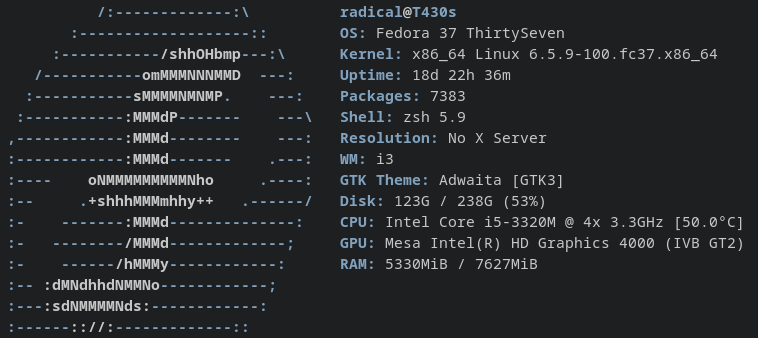
\includegraphics[width=0.8\textwidth]
	{linux_specs}
	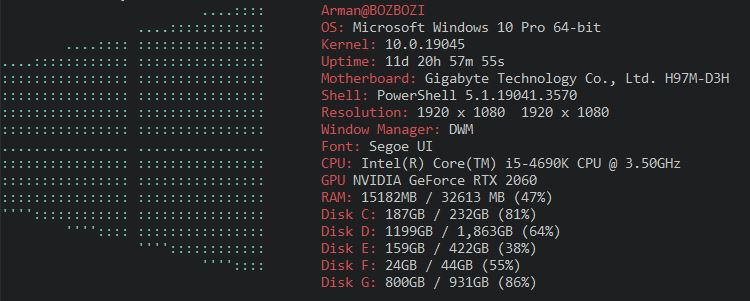
\includegraphics[width=0.8\textwidth]
	{windows_specs}
	\caption{Full system specifications of both Linux and Windows platforms}
\end{figure}

\subsection{Running the Implementation}
Our implementation's main entry point is a Python program file named \texttt{main.py}. The Python program takes an argument as input. We must first, as a command line argument, give it the path to a directory which contains all of the fingerprint pictures files within our dataset.
\begin{center}
	\texttt{python main.py D:$\backslash$path-to-directory$\backslash$}
\end{center}
Each file name must follow this format: \texttt{<finger\_id\_number>\_<finger\_impression\_number>.tiff}. For instance, \texttt{101\_4.tiff} is the fingerprint picture of the 4th impression of finger number 101.

After processing a whole dataset, the program saves all TFT data within a .npy file in the same directory as \texttt{main.py}. To obtain the matching score related results, we must run the \texttt{main.py} file again, but this time we must give it the path to our desired .npy file.
\begin{center}
	\texttt{python main.py D:$\backslash$path-to-file$\backslash$test.npy}
\end{center}

\subsection{The Advantages of our Implementation}
In comparison to the original implementation of the Yang method, our implementation possess two main advantages. For one, our implementation is fully free and open source. All the libraries, datasets, and frameworks we've used are completely free of charge and are available as open source repositories on GitHub or any other Git-related platforms. Thus the results within our paper can be easily verified by visiting our project's repository page and running our source code to obtain the same results.

The second advantage, is the capability of our code to utilize the GPU's CUDA cores for parallel processing and greatly improving our code's runtime performance to when only the CPU is utilized.

\chapter{Evaluation}
In this chapter, our sole focus will be on the algorithm's fingerprint matching accuracy, runtime performance, and memory usage. We will use the same exact fingerprint datasets used in the article for conducting our matching accuracy tests. Unfortunately, due to time constraints, it was not possible to conduct security related tests, such as testing ARM attack invulnerability, revocability, and unlinkability. 

Also the EERs we've obtained were nowhere close to the EERs obtained in the Yang paper. Even after weeks of investigation and fixing multiple typos in our implementation, the root cause of this deviation has not been found yet.

\section{Brief Introduction to Matching Metrics}
To determine the matching accuracy of any method, we need to first of all process a fingerprint dataset and derive all the matching scores between all possible pairs of fingerprints. Next, we'll declare a variable named the Acceptance Threshold $t_A$ which is ranged between 0 and 1. The use for this variable is to declare whether two fingerprints match each other and belong to the same finger or not. If a fingerprint pair's matching score is higher than $t_A$, then the fingerprint pair are considered to be matching each other and accepted as a result. If on the other hand, the matching score is lower than the threshold, the fingerprint pair is deemed as rejected.

\subsection{GAR, FAR, FRR, and EER}
A few important factors for deriving the matching accuracy of our method are the Genuine Acceptance Rate (GAR), False Acceptance Rate (FAR), False Rejection Rate (FRR), and Equal Error Rate (EER).

Under a certain Acceptance Threshold $t_A$, the GAR is the ratio of the number of accepted fingerprint pairs to the number of all fingerprint pairs taken from the same finger, otherwise known as genuine tests. The FAR is the ratio of the number of accepted fingerprints to the number of all fingerprint pairs taken from different fingers. The FRR is basically equal to 1-GAR.

As we can see, we can get different values for the GAR, FAR, and FRR under different acceptance threshold values. Therefore we can deduce that the GAR, FAR and FRR are essentially functions parametrized by $t_A$. Finally the EER's definition is as following:

\begin{center}
	If $t_A$ is such that: FAR($t_A$) = FRR($t_A$) then: EER = FAR($t_A$) = FRR($t_A$) 
\end{center}

By starting at 0 and incrementing $t_A$ by 0.001, we can eventually get to the point where the FRR and FAR meet. The lower the EER value, the more accurate our matching system is.

\section{Reliability of FingerFlow}
First we need to look into FingerFlow itself and see whether it works as intended and gives us the right minutiae to work with or not. One way to confirm this, would be to give FingerFlow a dataset of fingerprints, and then have it calculate the matching scores for every pair using its own built in method for matching. Then an ROC curve will have to be drawn based on its GAR and FAR.

Unfortunately, we haven't been able to utilize FingerFlow's matching functionality due to a lack of documentation and not having enough time to reverse engineer its source code to find out the appropriate input for its matching function. So the only thing we have to work with, is the developer's own ROC curve plot which is based off of an unknown fingerprint dataset, and multiple matching modules referred to as VerifyNet which come in different versions.

\begin{figure}[H]
	\centering
	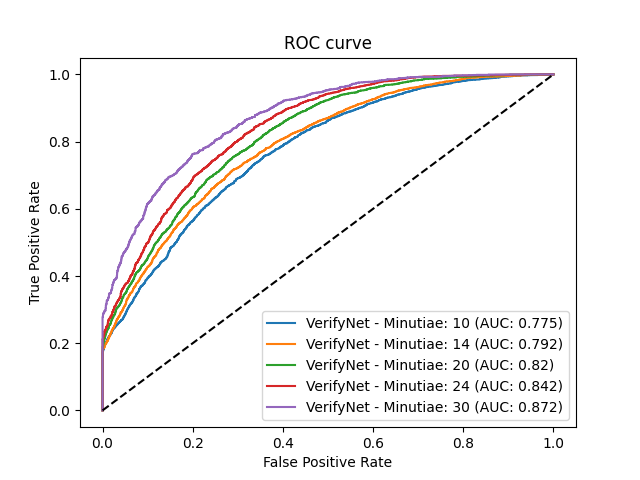
\includegraphics[width=0.8\textwidth]
	{fingerflow_roc}
	\caption{FingerFlow's ROC curve generated by different VerifyNet modules}
\end{figure}

Assuming this very limited information to be true, we can conclude that the deviation in the EERs obtained by our implementation, has less to do with FingerFlow itself, and may have to do with either an issue within the implementation itself, or it missing some vital factor in its entirety.

\section{Matching Accuracy of the Yang Method}
The fingerprint datasets used for this section are: FVC 2002 DB1, FVC 2002 DB2, FVC 2002 DB3, FVC 2004 DB4. Each of which include 80 fingerprint images in total, which are 8 different impressions of 10 different fingerprints. We also have two different protocols involved for the selection of fingerprint pairs. The default protocol considers the set of all pair selections from the whole dataset, but the 1V1 protocol only considers the set of all pair selections from the first two impressions of each fingerprint, resulting in a smaller dataset to work with.

\subsection{Case 1: Both Schemes vs. Delaunay Only vs. Polar Only}
In this section, under the 1V1 protocol performed on the FVC 2002 DB2 dataset, using the regular Feature Decorrelation Algorithm, and a projection matrix dimension $Y$ of 300, we are going to derive  three ROC curves from three instances where both schemes, only the delaunay scheme, and only the polar scheme was used for obtaining the final score. Below are the ROC curve figures on the paper compared to the one we derived from our implementation:

\begin{figure}[H]
	\centering
	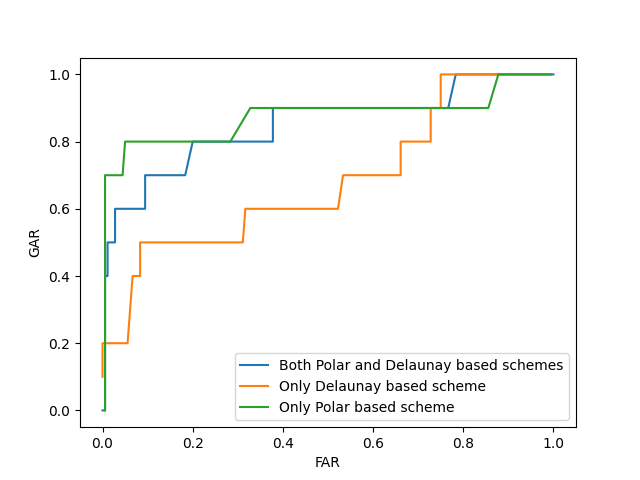
\includegraphics[width=0.45\textwidth]
	{3ROC}
	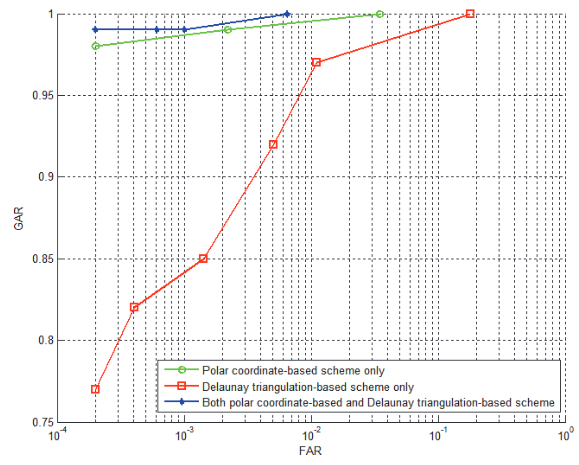
\includegraphics[width=0.45\textwidth]
	{3ROC2}
	\caption{The three ROC curves derived from our and the author's implementation}
\end{figure}

The resulting EERs we got from the three instances are as follows: Delaunay only EER = 0.400, Polar only EER = 0.197, Regular EER = 0.220.

\begin{figure}[H]
	\centering
	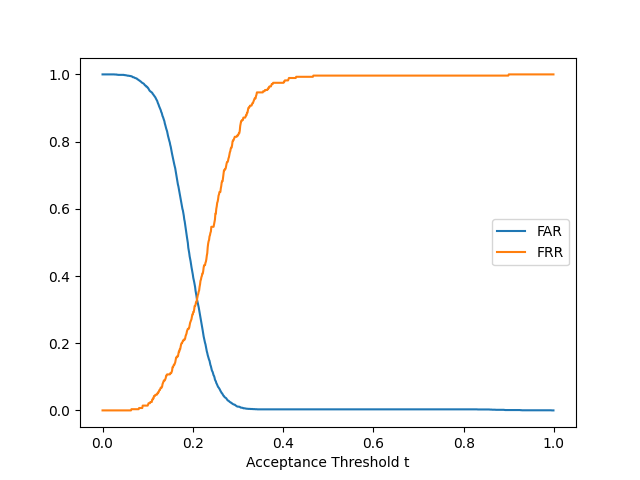
\includegraphics[width=0.45\textwidth]
	{FARFRR}
	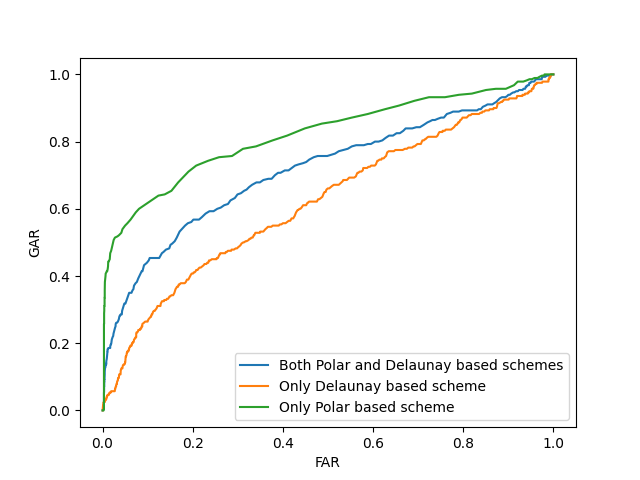
\includegraphics[width=0.45\textwidth]
	{33ROC}
	\caption{The ROC curves and FAR(t)/FRR(t) plots derived from Default protocol using the same dataset as above}
\end{figure}

\subsection{Case 2: Feature Decorrelation Algorithm Parameters}
In this test case we're going to see the effects of changing the parameters within both the enhanced and normal versions of the Feature Decorrelation Algorithm, namely $L_C$ and $L_S$. This will be done under the datasets FVC 2002 DB2 and FVC 2002 DB3, and the 1V1 protocol.


\begin{table}[H]
	\centering
\begin{tabular}{|lccc|}
	\hline
	\multicolumn{4}{|c|}{\cellcolor[HTML]{DAE8FC}Using Regular Feature Decorrelation Algorithm}                                                           \\ \hline
	\multicolumn{1}{|l|}{$L_C$}                       & \multicolumn{1}{c|}{20000}              & \multicolumn{2}{c|}{500}                                   \\ \hline
	\multicolumn{1}{|l|}{FVC2002 DB2}              & \multicolumn{1}{c|}{0.298}              & \multicolumn{2}{c|}{0.400}                                 \\ \hline
	\multicolumn{1}{|l|}{FVC2002 DB3}              & \multicolumn{1}{c|}{0.463}              & \multicolumn{2}{c|}{0.527}                                 \\ \hline
	\multicolumn{4}{|c|}{\cellcolor[HTML]{DAE8FC}\begin{tabular}[c]{@{}c@{}}Using Enhanced Feature Decorrelation Algorithm\\ and $L_C$ = 20000\end{tabular}} \\ \hline
	\multicolumn{1}{|l|}{$L_S$}                       & \multicolumn{1}{c|}{50}                 & \multicolumn{1}{c|}{5}                 & 1                 \\ \hline
	\multicolumn{1}{|l|}{FVC2002 DB2}              & \multicolumn{1}{c|}{0.230}              & \multicolumn{1}{c|}{0.220}             & 0.298             \\ \hline
	\multicolumn{1}{|l|}{FVC2002 DB3}              & \multicolumn{1}{c|}{0.234}              & \multicolumn{1}{c|}{0.300}             & 0.463             \\ \hline
\end{tabular}
	\caption{EERs derived from different parameters in both Feature Decorrelation Algorithms}
\end{table}

As it can be seen, the increase of EER is positively correlated with the increase in $L_S$ and decrease in $L_C$.

\subsection{Case 3: Random Projection Matrix Dimension}
In this test case we will compare the matching performance under different values of Random Projection matrix dimension $Y$. This will be done under the datasets FVC 2002 DB2 and FVC 2002 DB3, and the 1v1 protocol.


\begin{table}[H]
	\centering
	\begin{tabular}{|
			>{\columncolor[HTML]{DAE8FC}}l |l|l|}
		\hline
		Y           & 300   & 50    \\ \hline
		FVC2002 DB2 & 0.298 & 0.368 \\ \hline
		FVC2002 DB3 & 0.468 & 0.465 \\ \hline
	\end{tabular}
	\caption{EERs derived from different Y dimensions of the Random Projection Matrix}
\end{table}

\section{Runtime Performance}
This section is dedicated to comparing the runtime performances of different functions in our implementation. The average runtime lengths of these functions, under both the CPU only environment and the CUDA powered environment is described in the table below:

% Please add the following required packages to your document preamble:
% \usepackage[table,xcdraw]{xcolor}
% Beamer presentation requires \usepackage{colortbl} instead of \usepackage[table,xcdraw]{xcolor}
\begin{table}[H]
	\centering
	\begin{tabular}{|l|l|l|}
		\hline
		\rowcolor[HTML]{DAE8FC} 
		\multicolumn{1}{|c|}{\cellcolor[HTML]{DAE8FC}Function} & \multicolumn{1}{c|}{\cellcolor[HTML]{DAE8FC}Average CPU Runtime} & Average GPU Runtime \\ \hline
		Extraction of a Single Minutiae (FingerFlow)           & $\sim$350 ms                                                     & $\sim$60 ms         \\ \hline
		Extraction of all Minutiae in fingerprint (FingerFlow) & $\sim$65 s                                                       & $\sim$11 s          \\ \hline
		Random Projection Matrix Multiplication (Numba)        & $\sim$1.1 s                                                      & $\sim$0.1 s         \\ \hline
	\end{tabular}
	\caption{Table of Runtime Performance comparison}
\end{table}
As seen in the table above, GPU utilization has linearly improved our runtime performance in almost all cases. In case of small scale basic operations, there were no distinguishable change in performance in either environment.

As for the matching times, the author claims in their paper that finding the \texttt{SD} of a fingerprint pair takes around 0.00872 seconds, and finding each \texttt{SC} takes around 0.000171 seconds. If we assume each fingerprint has 20 minutiae on average, therefore each Polar TFT array has 20 vectors inside it. Hence calculating \texttt{SC\_MAX} would takr $20 \times 20 \times 0.000171 = 0.0684$ seconds in total.

In our implementation, calculating \texttt{SD} takes around 0.1 seconds on average when the size of our Delaunay TFT is $2^{20}$ bits, and 0.001 seconds when it is reduced to only 20000 bits. Calculating the \texttt{SC\_MAX} of a pair of fingerprints takes around 0.08 seconds on average altogether. It is safe to claim that our implementation's performance is superior to the original implementation by a good margin.

\section{Storage Requirement Comparison}
Here we will compare the storage size of the saved TFT data in our and the author's implementation. On average, the size of each of our NPY files, which would contain all the TFT of an entire dataset of 80 fingerprints, comes down to 180 MBs. That's around 2.25 MBs of disk space dedicated to both the Polar and Delaunay TFTs of a single fingerprint if the total file size is evenly distributed. Also note that NumPy also compresses the saved data before writing it to an output file, meaning that our file would be larger than 180 MBs on average if it weren't compressed. 

Some of this bloated size is because of the Delaunay TFT, which is $2^{20}$ bits or 128 KBs in size per Delaunay TFT of a fingerprint. If we reduce the Delaunay TFT size to 20000 bits or 2.4 KBs, we'd see a reduction of 125 KBs per fingerprint. Therefore for a database of 80 fingerprints, optimally only 192 KBs of data would be solely dedicated to the Delaunay TFTs, and only 9.7 MBs of space would be saved. Therefore, most of the bloat would be dedicated to the Polar TFT because it stores huge arrays with accurate complex valued entries for which the real and imaginary portions are both 32 bit floating point values.

What the author claims about their TFT sizes in their implementation, is that for a single fingerprint, the Delaunay TFT is around 20,000 bits or 2.5 KBs in size, and the Polar TFT takes close to 4.7 KBs per vector, for which if we assume that each fingerprint has an average of 20 minutiae, the total Polar TFT size amounts to roughly 94 KBs. In total the size of a single fingerprint's saved TFT data in the author's implementation is 96.5 KBs.

Overall, the storage requirement of our implementation can be greatly optimized if we were to reduce the accuracy of the complex values within the Polar TFT vectors. During runtime, the RAM usage is the same as the NPY file's size.
\chapter{Conclusion}
In the final chapter of this report, we will be discussing our achievements and what is left to be achieved in future versions of our implementation.

\section{What has been achieved}
In regards to the underlying concepts and theory of the Yang method article, I am satisfied to declare that I've almost entirely understood the intricacies of each procedure and concept within the paper and have managed to implement each of them to the best of my understandings and ability.

Other achievements in this project were the advantages discussed in 3.2.4 regarding the project being completely open source, and its capability to utilize an Nvidia GPU's CUDA cores for parallel processing, which opens up potential to further contributions to this project, and even others' collaboration in it.

I would claim that the greatest challenge in this project, was not the implementation of the method, but understanding the method itself despite there being a lot of ambiguity and vagueness within the explanations and descriptions of the 2018 paper. Fortunately, during the development period, I was able to get into contact with the main author of the 2018 paper, Dr. Wencheng Yang, and have him explain to me some of the details I've either missed out on or misunderstood. They were also considerate enough to share snippets of their MATLAB source codes via email, despite the closed source nature of their paper and its respective implementation.

\section{What is left to be achieved}
Some of the things that were left out as a result of our project's time constraints, which may be added in the future versions, include debugging, thorough documentation, and containerization of our implementation. 

Debugging would involve fixing the implementation and riding it of inaccuracies that cause the deviation in the achieved EER data. Thorough documentation would include the explanation behind every constant variable used in the implementation, and an installation manual for the implementation.

Unfortunately, as of now, it would be difficult for someone to run our implementation on their own machine, due to the intricate setup needed for it and a lack of installation instructions. Containerization with Docker is another viable solution to this, which would involve the user generating their own Docker image from a pre-written Dockerfile placed in the project repository, and creating a Docker container and running the code on it in an isolated environment.

Also there exist numerous fingerprint datasets online (on websites such as Kaggle) in addition to FVC datasets we've used in this project. Those would be a great addition to this project in future test cases.

\bibliographystyle{socreport}
\bibliography{socreport}

\appendix
\chapter{Code}
\section{Bowyer-Watson Pseudo-Code}
\label{code:a1}
\begin{lstlisting}
	def BowyerWatson (pointList):
		#pointList is a set of coordinates defining the points to be triangulated
		triangulation := empty triangle mesh data structure
		# must be large enough to completely contain all the points in pointList
		add super-triangle to triangulation 
		# add all the points one at a time to the triangulation
		for each point in pointList: 
			badTriangles := empty set
			# first find all the triangles that are no longer valid due to the insertion
			for each triangle in triangulation: 
				if point is inside circumcircle of triangle:
					add triangle to badTriangles
			polygon := empty set
			# find the boundary of the polygonal hole
			for each triangle in badTriangles: 
				for each edge in triangle:
					if edge is not shared by any other triangles in badTriangles:
						add edge to polygon
			# remove them from the data structure
			for each triangle in badTriangles:
				remove triangle from triangulation
			# re-triangulate the polygonal hole
			for each edge in polygon:
				newTri := form a triangle from edge to point
				add newTri to triangulation
		# done inserting points, now clean up
		for each triangle in triangulation:
			if triangle contains a vertex from original super-triangle:
				remove triangle from triangulation
		return triangulation
\end{lstlisting}

\end{document}
